\section{Anharmonicity}\label{sec:5.7}

The Raman line of the zone-center optical phonon of silicon is not infinitely sharp. Near zero temperature its full width at half maximum is \SI{1.45}{cm^{-1}}, or \SI{0.18}{meV}~\cite{menendez1984temperature}, so that a phonon created at \SI{64.1}{meV} survives for about \SI{3.7}{ps}, some sixty oscillations, before it disappears. The harmonic crystal of \cref{sec:5.2,sec:5.3} cannot account for this width. Its phonons are exact eigenstates of \cref{eq:5.3-Hb} and have infinite lifetime. The lifetime is limited by the part of the energy surface that the harmonic approximation dropped, the cubic term already visible in \cref{fig:5-scales}(c), which lets one phonon turn into two. For detection the decay matters: when a dark-matter particle creates an optical phonon in a cryogenic crystal, the phonon does not stay where it was made, and within picoseconds it splits into acoustic phonons, which carry the energy to the sensors on the surface (\cref{sec:20.2}). Every lattice response computed in this chapter is the leading term of an expansion in the anharmonic terms. Before trusting these responses, we need to know how large the anharmonic terms are.

\subsection{Cubic and quartic force constants}

The expansion \cref{eq:5.2-expand} of the energy surface continues beyond second order. With the compact label $i = (\vect{R}_i\kappa_i\alpha_i)$ for a nucleus and a Cartesian direction, so that $u_i = u^{\alpha_i}_{\vect{R}_i\kappa_i}$,
\begin{equation}
  \begin{gathered}
  E^{\mathrm{ad}}(u) = E^{\mathrm{ad}}(0) + \frac{1}{2!}\sum_{ij}\Phi^{(2)}_{ij}\,u_iu_j + \frac{1}{3!}\sum_{ijk}\Phi^{(3)}_{ijk}\,u_iu_ju_k
  \\
  {} + \frac{1}{4!}\sum_{ijkl}\Phi^{(4)}_{ijkl}\,u_iu_ju_ku_l + \cdots ,
  \\
  \Phi^{(n)}_{i_1\dots i_n} = \frac{\partial^nE^{\mathrm{ad}}}{\partial u_{i_1}\cdots\partial u_{i_n}}\bigg|_{u=0} .
  \end{gathered}
  \label{eq:5.7-expand}
\end{equation}
The \emph{third- and fourth-order force constants} $\Phi^{(3)}$ and $\Phi^{(4)}$ share the properties of $\Phi^{(2)}$ that \cref{sec:5.2} derived. As derivatives they are real and symmetric under any permutation of their labels. Since a lattice translation leaves the surface unchanged, they depend on the cells only through differences, $\Phi^{(3)}(\vect{R},\vect{R}',\vect{R}'') = \Phi^{(3)}(\vect{0},\vect{R}'-\vect{R},\vect{R}''-\vect{R})$. A rigid displacement of the whole crystal, $u_i \to u_i + d^{\alpha_i}$, also leaves the surface unchanged, so the total force $\sum_{\vect{R}\kappa}\partial E^{\mathrm{ad}}/\partial u^\gamma_{\vect{R}\kappa}$ vanishes at every configuration. Differentiating this identity $n - 1$ times at $u = 0$ gives the sum rules
\begin{equation}
  \sum_{\vect{R}''\kappa''}\Phi^{(n),\alpha\beta\cdots\gamma}_{\kappa\kappa'\cdots\kappa''}(\vect{R},\vect{R}',\dots,\vect{R}'') = 0 ,
  \label{eq:5.7-asr}
\end{equation}
of which \cref{eq:5.2-asr} is the case $n = 2$. Physically, $\Phi^{(3)}$ says how the force constants change when the nuclei move, $\Phi^{(2)}_{ij}(u) = \Phi^{(2)}_{ij} + \sum_k\Phi^{(3)}_{ijk}u_k + \cdots$, and $\Phi^{(4)}$ how that change changes in turn. The asymmetric curve of \cref{fig:5-scales}(c) is a direct measurement of one combination of the cubic constants: along the $[111]$ bond coordinate of silicon the cubic coefficient is $\Phi^{(3)}_{\mathrm{opt}} = \SI{-41.5}{eV.\angstrom^{-3}}$ (\cref{we:5-kappa}), and the quartic one is about $\SI{40}{eV.\angstrom^{-4}}$ (\cref{we:5-frozen}). A bond is stiffer under compression than under stretching: its force constant falls as it lengthens.

In practice the cubic constants come from the same calculations as the harmonic ones. By the $2n + 1$ theorem of \cref{sec:5.4}, the first-order density responses of DFPT fix the third derivatives of the energy, so that one set of linear-response calculations on a grid of wavevectors contains $\Phi^{(3)}$ as well~\cite[Eq.~(123)]{baroni2001phonons}. The alternative is finite differences of forces in a supercell, with one calculation for each symmetry-distinct pair of displaced atoms and a cutoff on the range of the triplets, or a fit to forces sampled at temperature $T$. The fourth-order constants are rarely computed term by term; they enter through the effective harmonic theories at the end of this section.

To see what the cubic term does to phonons, we write it in the phonon operators of \cref{sec:5.3}. When the phonon expansion \cref{eq:5.3-u} is inserted three times, each displacement brings a factor $(2NM_\kappa\omega)^{-1/2}$, a polarization vector, a phase and a displacement field. At fixed relative positions, summing the three phases over the first cell $\vect{R}$ gives $\sum_{\vect{R}}\ee^{\ii(\vect{Q}_1 + \vect{Q}_2 + \vect{Q}_3)\cdot\vect{R}} = N\sum_{\vect{G}}\delta_{\vect{Q}_1 + \vect{Q}_2 + \vect{Q}_3,\vect{G}}$, by the lattice sum \cref{eq:3.1-latticesum}. With the phonon labels written $1 = (\vect{Q}_1\nu_1)$ and so on,
\begin{equation}
  H_3 = \frac{1}{3!}\frac{1}{\sqrt N}\sum_{123}\sum_{\vect{G}}\delta_{\vect{Q}_1 + \vect{Q}_2 + \vect{Q}_3,\vect{G}}\,V^{(3)}(1,2,3)\,B_1B_2B_3 ,
  \label{eq:5.7-H3}
\end{equation}
with the \emph{three-phonon vertex}
\begin{equation}
  \begin{split}
  V^{(3)}(1,2,3) = {}& \frac{1}{\sqrt{8\,\omega_1\omega_2\omega_3}}\sum_{\kappa}\sum_{\vect{R}'\kappa'}\sum_{\vect{R}''\kappa''}\ee^{\ii(\vect{Q}_2\cdot\vect{R}' + \vect{Q}_3\cdot\vect{R}'')}
  \\ &\times \frac{\Phi^{(3),\alpha\beta\gamma}_{\kappa\kappa'\kappa''}(\vect{0},\vect{R}',\vect{R}'')\,e^\alpha_{\kappa\nu_1}(\vect{Q}_1)\,e^\beta_{\kappa'\nu_2}(\vect{Q}_2)\,e^\gamma_{\kappa''\nu_3}(\vect{Q}_3)}{\sqrt{M_\kappa M_{\kappa'}M_{\kappa''}}} ,
  \end{split}
  \label{eq:5.7-V3}
\end{equation}
summed over Cartesian indices, and $\omega_i = \omega_{\vect{Q}_i\nu_i}$. The vertex has the dimension of an energy and is symmetric in its three labels, and $V^{(3)}(-1,-2,-3) = V^{(3)}(1,2,3)^*$ by \cref{eq:A.6-e}. The factor $1/\sqrt N$ comes from spreading three phonons over the whole crystal, and the Kronecker delta is the conservation of crystal momentum: three phonons can meet only if their wavevectors add up to a reciprocal-lattice vector. Since each $B_i$ creates or destroys one phonon, $H_3$ turns one phonon into two, two into one, or creates or destroys three at once. The quartic term, written in the same way, has four fields and the factor $1/N$.

\subsection{Three-phonon decay and the linewidth}

Consider a crystal in thermal equilibrium, except for a small excess population in one mode $\vect{Q}\nu$. Since $\omega_{\vect{Q}\nu} > 0$, the processes of $H_3$ that conserve energy are of two kinds. The phonon can decay into two others, $\vect{Q}\nu \to 1 + 2$, or merge with a thermal phonon into a third, $\vect{Q}\nu + 1 \to 2$. For the decay, the matrix element of \cref{eq:5.7-H3} between $|n_{\vect{Q}\nu}, n_1, n_2\rangle$ and $|n_{\vect{Q}\nu} - 1, n_1 + 1, n_2 + 1\rangle$ comes from the terms that contain $b_{\vect{Q}\nu}$, $b^\dagger_1$ and $b^\dagger_2$. These three operators are in $B_{\vect{Q}\nu}$, $B_{-1}$ and $B_{-2}$, with $-1 = (-\vect{Q}_1\nu_1)$, and there are $3!$ ways of assigning the three fields to the three slots of $H_3$, all equal by the symmetry of the vertex. The $3!$ cancels, and the boson factors of \cref{eq:2.3-boson} give
\begin{equation*}
  \langle n_{\vect{Q}\nu} - 1, n_1 + 1, n_2 + 1|H_3|n_{\vect{Q}\nu}, n_1, n_2\rangle = \frac{V^{(3)}(\vect{Q}\nu,-1,-2)}{\sqrt N}\,\sqrt{n_{\vect{Q}\nu}(n_1 + 1)(n_2 + 1)} ,
\end{equation*}
with $\vect{Q}_1 + \vect{Q}_2 = \vect{Q}$ up to a reciprocal-lattice vector. By the golden rule \cref{eq:2.1-golden}, the rate at which the mode loses phonons this way is $(2\pi/N)\sum|V^{(3)}|^2n_{\vect{Q}\nu}(n_1 + 1)(n_2 + 1)\,\delta(\omega_{\vect{Q}\nu} - \omega_1 - \omega_2)$, summed over distinct final pairs, a sum that is half the sum over $\vect{Q}_1$, $\nu_1$ and $\nu_2$ with $\vect{Q}_2$ fixed. The inverse process, in which the pair merges back, feeds the mode at the rate with $(n_{\vect{Q}\nu} + 1)n_1n_2$ in place of $n_{\vect{Q}\nu}(n_1 + 1)(n_2 + 1)$. The difference of the two occupation factors is $n_{\vect{Q}\nu}(1 + n_1 + n_2) - n_1n_2$. At equilibrium this difference vanishes, since $n_{\mathrm{B}}(\omega_1 + \omega_2)(1 + n_1 + n_2) = n_1n_2$ for Bose functions, the detailed-balance condition for the process (\cref{sec:2.5}). For an excess $\delta n$ in the mode the difference is $(1 + n_1 + n_2)\,\delta n$, so the excess decays exponentially. The merging processes contribute in the same way, with the occupation difference $n_{\vect{Q}\nu}n_1(1 + n_2) - (n_{\vect{Q}\nu} + 1)(n_1 + 1)n_2 = (n_1 - n_2)\,\delta n$, and with no factor one half, since the two partners now play different roles. After the relabeling $\vect{Q}_i \to -\vect{Q}_i$, which leaves $\omega_i$ and $n_i$ unchanged, the decay and merging terms add, and the excess decays as $\ee^{-\gamma^{\mathrm{anh}}_{\vect{Q}\nu}t}$ with
\begin{keyresult}[Three-phonon linewidth]
\begin{equation}
  \begin{split}
  \gamma^{\mathrm{anh}}_{\vect{Q}\nu} = {}& \frac{\pi}{N}\sum_{\vect{Q}_1\nu_1\nu_2}\bigl|V^{(3)}(\vect{Q}\nu,\vect{Q}_1\nu_1,\vect{Q}_2\nu_2)\bigr|^2
  \\ &\times\Bigl[(1 + n_1 + n_2)\,\delta(\omega_{\vect{Q}\nu} - \omega_1 - \omega_2) + 2(n_1 - n_2)\,\delta(\omega_{\vect{Q}\nu} + \omega_1 - \omega_2)\Bigr] ,
  \end{split}
  \label{eq:5.7-gamma}
\end{equation}
with $\vect{Q}_2 = -\vect{Q} - \vect{Q}_1$ up to a reciprocal-lattice vector, $\omega_i = \omega_{\vect{Q}_i\nu_i}$ and $n_i = n_{\mathrm{B}}(\omega_i)$. The first term is the decay of the phonon into the pair $(-\vect{Q}_1\nu_1, -\vect{Q}_2\nu_2)$, the second its merging with $\vect{Q}_1\nu_1$ into $-\vect{Q}_2\nu_2$.
\end{keyresult}
This is the result of Maradudin and Fein~\cites{maradudin1962scattering}[Eq.~(6)]{paulatto2013anharmonic}. The rate at which an excess population relaxes is also the width of the line. A state that decays with probability $\ee^{-\gamma t}$ has an amplitude that decays as $\ee^{-\gamma t/2}$, and its spectrum is a Lorentzian with full width $\gamma$ at half maximum. The \emph{phonon linewidth} $\gamma_{\vect{Q}\nu}$ is this full width, the inverse lifetime of the phonon, and $\gamma^{\mathrm{anh}}_{\vect{Q}\nu}$ is its anharmonic part; in the language of the phonon self-energy of \cref{sec:6.4}, defined there in units of a squared frequency, $\gamma^{\mathrm{anh}}_{\vect{Q}\nu}$ is $-\Imag\Pi_\nu/\omega_{\vect{Q}\nu}$ for the bubble with two cubic vertices. Other mechanisms add to the linewidth: the creation of electron--hole pairs, $\gamma^{\mathrm{ep}}_{\vect{Q}\nu}$, which vanishes in an insulator at zero temperature (\cref{sec:6.4}), and the scattering by isotopes and defects (\cref{sec:11.6}).

\Cref{eq:5.7-gamma} has two ingredients, the strength of the vertex and the number of pairs that conserve energy and crystal momentum, and the second is often the more restrictive. Temperature enters only through the occupations. At $T = 0$ only spontaneous decay remains, with weight one: a phonon of a cryogenic crystal can split, but it finds no thermal phonon to merge with. At high temperature $n_i \approx T/\omega_i$, and the width grows linearly with $T$.

The zone-center optical phonon of silicon is a concrete case. Since its wavevector is zero, it decays into pairs with opposite wavevectors, $(\vect{Q}_1, -\vect{Q}_1)$, and their energies must add to $\omega_{\mathrm{opt}} = \omega_{\mathrm{\Gamma},\mathrm{opt}}$. It is also the highest phonon of the crystal and has no partner to merge with, so only the decay term of \cref{eq:5.7-gamma} contributes, at any temperature. \Cref{fig:5-decay}(a) shows the allowed pairs on the computed dispersion as crossings between a branch and the mirror image $\omega_{\mathrm{opt}} - \omega_{\vect{Q}\nu}$ of another. Klemens proposed the simplest channel: two acoustic phonons of the same branch, each with energy $\omega_{\mathrm{opt}}/2$~\cite{klemens1966anharmonic}. With $\omega_1 = \omega_2 = \omega_{\mathrm{opt}}/2$ in \cref{eq:5.7-gamma} the occupation factor is the same for every pair, and the width follows the \emph{Klemens law}
\begin{equation}
  \gamma^{\mathrm{anh}}_{\mathrm{\Gamma},\mathrm{opt}}(T) = \gamma^{\mathrm{anh}}_{\mathrm{\Gamma},\mathrm{opt}}(0)\,\Bigl[1 + 2n_{\mathrm{B}}\Bigl(\frac{\omega_{\mathrm{opt}}}{2}\Bigr)\Bigr] .
  \label{eq:5.7-klemens}
\end{equation}
In silicon the Klemens channel is only partly open. The transverse acoustic branches never reach $\omega_{\mathrm{opt}}/2$: in the PBE calculation of \cref{fig:5-decay} they top out at \SI{26.4}{meV}, below $\omega_{\mathrm{opt}}/2 = \SI{31.8}{meV}$, and two transverse phonons cannot share the energy. Two longitudinal acoustic phonons can. However, few modes lie near $\omega_{\mathrm{opt}}/2$, where the phonon density of states is small. Most of the phase space is in asymmetric pairs, a transverse acoustic phonon near \SI{22}{meV} with a longitudinal one near \SI{42}{meV}, which make up \SI{89}{\percent} of the density of final states in \cref{fig:5-decay}(b), against \SI{7}{\percent} for the pairs of longitudinal phonons. A full DFPT calculation of the vertex finds the same ordering, \SI{94.3}{\percent} and \SI{5.7}{\percent}~\cite[Table~1]{debernardi1994anharmonic}. For asymmetric pairs the occupation factor $1 + n_1 + n_2$ is larger than Klemens's at the same temperature, because the softer partner is populated first (\cref{fig:5-decay}(c)).

\begin{figure}[tbp]
  \centering
  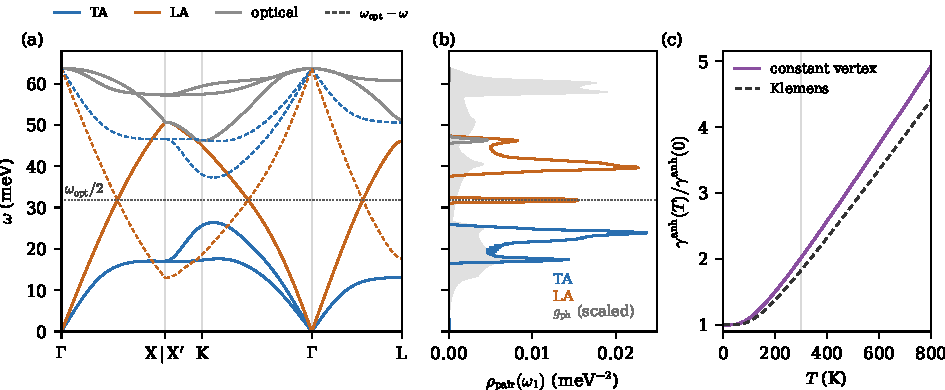
\includegraphics[width=\linewidth]{figures/ch05/fig5_6.pdf}
  \caption{Three-phonon decay of the zone-center optical phonon of silicon, $\omega_{\mathrm{opt}} = \SI{63.7}{meV}$ in this calculation. Phonons from the PBE force constants of \cref{fig:5-si} (DFPT on a $6^3$ grid of wavevectors, $a = \SI{5.431}{\angstrom}$), Fourier-interpolated; branches are labeled by energy order, the lowest two transverse acoustic (TA, blue), the third longitudinal acoustic (LA, orange), the upper three optical (gray). (a) Dispersion (solid) and the mirror curves $\omega_{\mathrm{opt}} - \omega_{\vect{Q}\nu}$ of the acoustic branches (dashed). A solid branch crossing a dashed one marks a pair $(\vect{Q},-\vect{Q})$ whose energies add to $\omega_{\mathrm{opt}}$; dotted: $\omega_{\mathrm{opt}}/2$. (b) Two-phonon density of final states resolved by the energy $\omega_1$ of one member of the pair and by its branch, $\rho_{\mathrm{pair}}(\omega_1) = N^{-1}\sum_{\vect{Q}\nu_1\nu_2}\delta(\omega_1 - \omega_{\vect{Q}\nu_1})\,\delta(\omega_{\mathrm{opt}} - \omega_{\vect{Q}\nu_1} - \omega_{\vect{Q}\nu_2})$, on an $80^3$ grid with Gaussians of width \SI{0.25}{meV} and a \SI{0.9}{meV} running mean; it is symmetric about $\omega_{\mathrm{opt}}/2$, each TA phonon (blue) pairing with an LA phonon (orange) at the mirror energy. Shaded: the one-phonon density of states $g_{\mathrm{ph}}$, scaled. LA+TA pairs make up \SI{89}{\percent} of the final states, LA+LA \SI{7}{\percent}, and TA+TA none; the remaining \SI{4}{\percent} are optical+TA pairs from a small region near K. (c) Temperature dependence of the width relative to $T = 0$: Klemens's law \cref{eq:5.7-klemens} (dashed) and the average of $1 + n_1 + n_2$ over the final states of panel (b) (solid), which assumes a constant vertex; the vertical line marks \SI{300}{K}.}
  \label{fig:5-decay}
\end{figure}

\begin{workedexample}{Klemens decay of the optical phonon of silicon}\label{we:5-klemens}
We compare the width of the zone-center optical phonon with the Klemens law \cref{eq:5.7-klemens}, using the measured $\omega_{\mathrm{opt}} = \SI{64.1}{meV}$.

\emph{The measured width.} At low temperature the Raman line of the mode has a full width of \SI{1.45}{cm^{-1}}~\cite{menendez1984temperature}, as tabulated in Ref.~\cite[Table~1]{debernardi1994anharmonic}. With $\SI{1}{cm^{-1}} = \SI{0.12398}{meV}$, this is $\gamma_{\mathrm{\Gamma},\mathrm{opt}} = \SI{0.180}{meV}$, and
\begin{equation*}
  \frac{\gamma_{\mathrm{\Gamma},\mathrm{opt}}}{\omega_{\mathrm{opt}}} = 2.80\times10^{-3} , \qquad
  \frac{1}{\gamma_{\mathrm{\Gamma},\mathrm{opt}}} = \SI{3.66}{ps} ,
\end{equation*}
57 periods of \SI{64.5}{fs}. Other measurements range from 1.24 to \SI{2.1}{cm^{-1}}~\cite{debernardi1994anharmonic}, a spread that reflects sample quality and spectral resolution. Silicon is an insulator, with $\gamma^{\mathrm{ep}}_{\vect{Q}\nu} = 0$ at low temperature, and isotope scattering is weak for a mode at the top of the spectrum. The width is anharmonic. A DFPT calculation of the full vertex \cref{eq:5.7-V3}, inserted in \cref{eq:5.7-gamma}, yields \SI{1.43}{cm^{-1}}~\cite[Table~1]{debernardi1994anharmonic}, \SI{99}{\percent} of the measured value, so three-phonon decay accounts for the whole width.

\emph{The temperature dependence.} At the \SI{10}{mK} of a detector, $\omega_{\mathrm{opt}}/2T = 3.7\times10^4$, the occupation $n_{\mathrm{B}}(\omega_{\mathrm{opt}}/2)$ is $\ee^{-37000}$, and the width is its zero-temperature value: the optical phonon decays spontaneously, with no help from thermal phonons. At \SI{77}{K}, $n_{\mathrm{B}}(\omega_{\mathrm{opt}}/2) = 0.008$ and the Klemens factor is 1.016. At \SI{300}{K}, $n_{\mathrm{B}}(\omega_{\mathrm{opt}}/2) = 0.407$, and \cref{eq:5.7-klemens} predicts
\begin{equation*}
  \gamma_{\mathrm{\Gamma},\mathrm{opt}}(\SI{300}{K}) = \SI{1.45}{cm^{-1}}\times(1 + 2\times0.407) = \SI{2.63}{cm^{-1}} .
\end{equation*}
With a constant vertex, averaging $1 + n_1 + n_2$ over the dominant asymmetric pairs gives a factor 2.01 instead of 1.82 and a width of \SI{2.92}{cm^{-1}} (\cref{fig:5-decay}(c)). The Klemens law thus gets the form of the temperature dependence right: a constant plus a term that grows as the Bose function of the daughters. Its single daughter energy, $\omega_{\mathrm{opt}}/2$, misses the true pairs of silicon, and at room temperature the Klemens law gives a width about \SI{10}{\percent} below the estimate from those pairs. With the full vertex and the true daughters, \cref{eq:5.7-gamma} follows the measured widths up to temperatures of the order of $\omega_{\mathrm{opt}} \approx \SI{740}{K}$~\cite{debernardi1994anharmonic}.

The Klemens law is a good parametrization of the temperature dependence once its zero-temperature width is taken from experiment or from a calculation. It does not predict that width, and its picture of the channel is wrong in silicon.
\end{workedexample}

\subsection{The anharmonic small parameter}

How large are the anharmonic terms compared with the harmonic ones? The natural measure is the ratio of the cubic to the harmonic energy at the zero-point amplitude of a mode. Take a bond-like coordinate with curvature $\Phi^{(2)}$, cubic coefficient $\Phi^{(3)}$ and zero-point length $\ell_{\mathrm{zp}}$. The ratio of $\tfrac16\Phi^{(3)}\ell_{\mathrm{zp}}^3$ to $\tfrac12\Phi^{(2)}\ell_{\mathrm{zp}}^2$ defines the \emph{anharmonic small parameter}
\begin{equation}
  \eta_{\mathrm{anh}} = \frac{|\Phi^{(3)}|\,\ell_{\mathrm{zp}}}{3\,\Phi^{(2)}} .
  \label{eq:5.7-eta}
\end{equation}
Equivalently, $\eta_{\mathrm{anh}}$ is the zero-point amplitude measured in units of the length $3\Phi^{(2)}/|\Phi^{(3)}|$ over which the force constants change by their own size. The counting of \cref{sec:5.1} estimates it at once. Force constants of every order scale as $\Phi^{(n)} \sim \alpha^2m_e/a_0^n$, and the zero-point amplitude as $\ell_{\mathrm{zp}} \sim \kappa_{\mathrm{BO}}a_0$, so
\begin{equation*}
  \eta_{\mathrm{anh}} \sim \frac{\alpha^2m_e/a_0^3}{\alpha^2m_e/a_0^2}\,\kappa_{\mathrm{BO}}a_0 = \kappa_{\mathrm{BO}} .
\end{equation*}
The anharmonic parameter is the Born--Oppenheimer parameter itself: the cubic term is smaller than a phonon energy by one power of $\kappa_{\mathrm{BO}}$, as \cref{sec:5.1} found. The quartic term, $\tfrac1{24}\Phi^{(4)}\ell_{\mathrm{zp}}^4$, is smaller than the harmonic one by $\eta_{\mathrm{anh}}^2$, since $\Phi^{(4)}\ell_{\mathrm{zp}}^2/\Phi^{(2)} \sim (\ell_{\mathrm{zp}}/a_0)^2$, and each further order brings one more power.

The physical effects follow by counting powers of $\eta_{\mathrm{anh}}$. The cubic term changes no energy at first order, since it is a product of an odd number of displacements and its average over any harmonic state vanishes. At second order it shifts the levels by $(\eta_{\mathrm{anh}}\omega_{\mathrm{ph}})^2/\omega_{\mathrm{ph}} = \eta_{\mathrm{anh}}^2\omega_{\mathrm{ph}}$, since the energy denominators of second-order perturbation theory are themselves phonon energies. The quartic term shifts them at first order by the same amount, $\eta_{\mathrm{anh}}^2\omega_{\mathrm{ph}}$. The decay rate \cref{eq:5.7-gamma} is the square of a cubic matrix element of size $\eta_{\mathrm{anh}}\omega_{\mathrm{ph}}$ times a density of final states of order $1/\omega_{\mathrm{ph}}$, again $\eta_{\mathrm{anh}}^2\omega_{\mathrm{ph}}$. The three effects are of one order:
\begin{equation}
  \frac{\gamma^{\mathrm{anh}}_{\vect{Q}\nu}}{\omega_{\vect{Q}\nu}} \sim \frac{\Delta\omega^{\mathrm{anh}}_{\vect{Q}\nu}}{\omega_{\vect{Q}\nu}} \sim \eta_{\mathrm{anh}}^2 \sim \kappa_{\mathrm{BO}}^2 ,
  \label{eq:5.7-order}
\end{equation}
where $\Delta\omega^{\mathrm{anh}}_{\vect{Q}\nu}$ is the anharmonic shift of the frequency. In absolute terms the shift and the width are $\alpha^2m_e\,\kappa_{\mathrm{BO}}^4$, the anharmonic level of the Born--Oppenheimer hierarchy of \cref{sec:5.1}. In the labeling of \cref{sec:8.5} the order $\eta_{\mathrm{anh}}^2$ is anharmonic order $n_A = 2$, where $n_A$ counts powers of the anharmonic expansion parameter in the response rather than vertices, and the leading anharmonic phonon self-energy is of that order. In thermal equilibrium the zero-point length is replaced by the thermal amplitude, $\ell_{\mathrm{zp}}^2 \to \ell_{\mathrm{zp}}^2(2n_{\mathrm{B}} + 1)$, as in \cref{eq:5.3-B}, and at high temperature $\eta_{\mathrm{anh}}^2$ grows in proportion to $T$, as the widths do.

Silicon bears out this counting. Along the bond coordinate of \cref{fig:5-scales}(c), $\Phi^{(2)} = \SI{13.6}{eV.\angstrom^{-2}}$, $\Phi^{(3)} = \SI{-41.5}{eV.\angstrom^{-3}}$ and $\ell_{\mathrm{zp}} = \SI{0.048}{\angstrom}$ give $\eta_{\mathrm{anh}} = 0.049$, against $\kappa_{\mathrm{BO}} = 0.067$; the length over which the force constants change is $3\Phi^{(2)}/|\Phi^{(3)}| = \SI{0.98}{\angstrom}$, about \SI{40}{\percent} of the bond. Then $\eta_{\mathrm{anh}}^2 = 2.4\times10^{-3}$. The quartic-to-harmonic ratio at the same amplitude, $\Phi^{(4)}\ell_{\mathrm{zp}}^2/12\Phi^{(2)}$ with $\Phi^{(4)} \approx \SI{40}{eV.\angstrom^{-4}}$, is $0.6\times10^{-3}$, a quarter of $\eta_{\mathrm{anh}}^2$, and the measured width of \cref{we:5-klemens} is $\gamma/\omega_{\mathrm{opt}} = 2.8\times10^{-3}$, 1.2 times $\eta_{\mathrm{anh}}^2$. The coefficients of the counting are close to one, between a quarter and two here and in the Born--Oppenheimer hierarchy of \cref{we:5-kappa}. Silicon at detector temperatures is a weakly anharmonic crystal, and its harmonic phonons are correct to a few parts in a thousand, well below the few-percent error of the functional (\cref{sec:5.2}).

The anharmonic parameter is not always small, and it grows with $\ell_{\mathrm{zp}}$. Light atoms have larger amplitudes, since $\ell_{\mathrm{zp}} \propto M^{-1/4}$ at fixed force constants, and hydrogen has $\kappa_{\mathrm{BO}} = 0.15$. The parameter also grows for soft modes near a structural instability, where $\Phi^{(2)} \to 0$ and the harmonic expansion about the minimum loses its meaning. The parameter is also large in quantum crystals such as solid helium, where the zero-point motion is a sizable fraction of the spacing, and in any crystal near melting. At low energy phonon decay is controlled by phase space rather than by $\eta_{\mathrm{anh}}$. The width of a long-wavelength acoustic phonon at $T = 0$ scales as the fifth power of its energy, and this width sets how fast the phonons that a dark-matter event leaves behind down-convert. For the nuclear response to dark matter, $\eta_{\mathrm{anh}}$ measures how far the harmonic results of this chapter can be trusted, and \cref{sec:11.5} turns it into a correction.

\subsection{Effective harmonic theories}

When temperature, light atoms or soft modes make the expansion \cref{eq:5.7-expand} converge slowly, the usual remedy is not to add orders but to find a better harmonic problem. Three effective harmonic theories are in common use, and they differ in what the harmonic force constants are fitted to.

The \emph{quasi-harmonic approximation} fits the force constants to the volume. It keeps every mode harmonic but computes the frequencies at the cell volume $\Omega$ that minimizes the free energy at temperature $T$, \cref{eq:E.8-qha}. The volume dependence of the frequencies is itself a cubic effect. A homogeneous strain $\epsilon$ displaces every nucleus by $u_i = \sum_\beta\epsilon^{\alpha_i\beta}X^\beta_i$, with $\vect{X}_i$ its equilibrium position. The force constants about the strained configuration then change, to first order, by
\begin{equation}
  \Phi^{(2)}_{ij}(\epsilon) - \Phi^{(2)}_{ij} = \sum_k\Phi^{(3)}_{ijk}\sum_\beta\epsilon^{\alpha_k\beta}X^\beta_k .
  \label{eq:5.7-strain}
\end{equation}
The Grüneisen parameter $\gamma^{\mathrm{G}}_{\vect{Q}\nu} = -\partial\ln\omega_{\vect{Q}\nu}/\partial\ln\Omega$ of \cref{sec:5.2} is therefore a projection of $\Phi^{(3)}$, and a harmonic crystal, with $\Phi^{(3)} = 0$, neither expands when heated nor shifts its phonons under pressure. The zero-point energy of \cref{sec:5.3} also depends on the volume, and the resulting zero-point pressure expands the lattice at $T = 0$ beyond the static minimum of \cref{sec:5.1}. The quasi-harmonic approximation keeps the cubic term at the level of the volume. It drops the shifts at fixed volume, which \cref{eq:5.7-order} puts at the same order, and it has no widths.

The \emph{self-consistent harmonic approximation} (SCHA) fits the force constants to the distribution of the nuclei, by a variational principle~\cite{errea2014anharmonic}. For any trial density matrix $\tilde\varrho$, the functional $\mathcal{F}[\tilde\varrho] = \langle H\rangle_{\tilde\varrho} - TS_{\mathrm{ent}}[\tilde\varrho]$ is an upper bound on the free energy (the Gibbs--Bogoliubov inequality). The SCHA takes for $\tilde\varrho$ the thermal state of a harmonic Hamiltonian $H_{\mathrm{trial}}$ with centroids $\bar X_a$ and auxiliary force constants $\Phi^{(2)}_{\mathrm{aux}}$, \cref{eq:E.8-scha}, with $a$ running over the Cartesian coordinates $X_a$ of all nuclei and $\delta X_a = X_a - \bar X_a$. The distribution of positions in this state is a Gaussian centered at $\bar X$. With $\mathcal{F}_{\mathrm{trial}}$ the free energy of $H_{\mathrm{trial}}$ and $V_{\mathrm{trial}} = \tfrac12\sum_{ab}\delta X_a\Phi^{(2)}_{\mathrm{aux},ab}\delta X_b$ its potential, the bound reads
\begin{equation*}
  \mathcal{F}[\tilde\varrho] = \mathcal{F}_{\mathrm{trial}} + \bigl\langle E^{\mathrm{ad}} - V_{\mathrm{trial}}\bigr\rangle_{\tilde\varrho} .
\end{equation*}
We minimize the bound. A change of $\Phi^{(2)}_{\mathrm{aux},ab}$ changes $\mathcal{F}_{\mathrm{trial}}$ by $\tfrac12\langle\delta X_a\delta X_b\rangle\,\delta\Phi^{(2)}_{\mathrm{aux},ab}$, the thermal form of the Hellmann--Feynman theorem of \cref{sec:5.1}, and the average of $V_{\mathrm{trial}}$ by the same amount plus $\tfrac12\sum_{cd}\Phi^{(2)}_{\mathrm{aux},cd}\,\delta\langle\delta X_c\delta X_d\rangle$. The first contributions cancel. The average of $E^{\mathrm{ad}}$ over a Gaussian depends on the force constants only through the covariance $\langle\delta X_c\delta X_d\rangle$, and a Gaussian obeys the diffusion equation in its covariance, so that $\delta\langle E^{\mathrm{ad}}\rangle = \tfrac12\sum_{cd}\langle\partial_c\partial_dE^{\mathrm{ad}}\rangle\,\delta\langle\delta X_c\delta X_d\rangle$. Altogether
\begin{equation*}
  \delta\mathcal{F} = \frac12\sum_{cd}\Bigl[\bigl\langle\partial_c\partial_dE^{\mathrm{ad}}\bigr\rangle_{\tilde\varrho} - \Phi^{(2)}_{\mathrm{aux},cd}\Bigr]\,\delta\langle\delta X_c\delta X_d\rangle ,
\end{equation*}
and the centroids enter only through $\langle E^{\mathrm{ad}}\rangle$, whose derivative is the average force. Both variations vanish at the minimum:
\begin{keyresult}[Self-consistent harmonic approximation]
\begin{equation}
  \Phi^{(2)}_{\mathrm{aux},ab} = \Bigl\langle\frac{\partial^2E^{\mathrm{ad}}}{\partial X_a\,\partial X_b}\Bigr\rangle_{\tilde\varrho} , \qquad
  \Bigl\langle\frac{\partial E^{\mathrm{ad}}}{\partial X_a}\Bigr\rangle_{\tilde\varrho} = 0 .
  \label{eq:5.7-scha}
\end{equation}
The auxiliary force constants are the curvature of the true energy surface averaged over the Gaussian distribution that they themselves generate, and the centroids lie where the average force vanishes.
\end{keyresult}
These are the stationarity conditions of Ref.~\cite[Eqs.~(21) and~(22)]{errea2014anharmonic}, which writes them as averages of forces. The first condition is self-consistent because the width of the distribution, $\langle\delta X_a\delta X_b\rangle$, is computed from the auxiliary frequencies with the zero-point and thermal factors of \cref{eq:5.3-B}. Expanded in the force constants, the average curvature is $\Phi^{(2)} + \tfrac12\sum_{cd}\Phi^{(4)}_{abcd}\langle\delta X_c\delta X_d\rangle + \cdots$: its first correction is the first-order quartic shift of \cref{eq:5.7-order}, and the SCHA sums this shift to all orders, together with the corrections from the higher even force constants. The cubic term enters only through the shift of the centroids and, in the physical phonon frequencies, through an added bubble term. For soft modes the SCHA is the right starting point even when the harmonic frequencies are imaginary, since the average curvature can be positive where the curvature at the minimum is not.

The \emph{temperature-dependent effective potential} fits the force constants to forces. It samples nuclear configurations at temperature $T$, by molecular dynamics, computes the forces in each, and finds the effective constants $\tilde\Phi^{(2)}$ that reproduce them best in the least-squares sense, \cref{eq:E.8-tdep}~\cite{hellman2011lattice}. For a Gaussian sample the least-squares fit returns exactly the average curvature of \cref{eq:5.7-scha}. The reason is that a Gaussian average of the force times a displacement is the average of the force's derivative times the covariance. The temperature-dependent effective potential and the SCHA differ in the distribution they sample, a classical one in molecular dynamics and a quantum Gaussian in the SCHA. That difference matters at detector temperatures, where a classical sample sees an almost static lattice and misses the zero-point motion. The same fit extends to effective third-order constants, from which \cref{eq:5.7-gamma} gives temperature-dependent widths~\cite{hellman2013temperature}.

For silicon at \SI{10}{mK}, all three effective harmonic theories reduce to the harmonic phonons of \cref{sec:5.2} with corrections of a few parts in a thousand, so the rest of the book can work with the harmonic phonons.

\section*{Summary}

Electrons are lighter than nuclei by a factor of about $2\times10^{-5}$ in silicon, and they settle into their ground state many times during one vibration of the lattice (\cref{sec:5.1}). The Born--Oppenheimer approximation turns their ground-state energy at fixed nuclei, with the repulsion of the nuclei added, into the potential-energy surface $E^{\mathrm{ad}}(u)$ on which the nuclei move. The small parameter is the fourth root of the mass ratio, $\kappa_{\mathrm{BO}} = (m_e/M)^{1/4} = 0.067$; in an insulator the ratio that controls the approximation is the phonon energy over the gap, 0.0548 in silicon.

Expanded to second order about its minimum, the energy surface defines the force constants $\Phi^{(2)}$ and the dynamical matrix $D^{\mathrm{dyn}}(\vect{Q})$, whose eigenvalues are the squared phonon frequencies $\omega^2_{\vect{Q}\nu}$ and whose eigenvectors are the polarizations $\vect{e}_{\kappa\nu}(\vect{Q})$ (\cref{sec:5.2}). Silicon has six branches up to \SI{64.1}{meV}, flat transverse acoustic branches that pile up states near \SI{17}{meV}, and no LO--TO splitting.

Quantized, each normal mode is an oscillator and a phonon is one of its quanta (\cref{sec:5.3}). Emitting a phonon has the weight $n_{\vect{Q}\nu} + 1$ and absorbing one the weight $n_{\vect{Q}\nu}$, and in a cryogenic detector every mode is empty, so emission is the whole signal. Zero-point motion alone spreads a silicon nucleus over \SI{0.05}{\angstrom} per Cartesian component.

In a polar crystal the sublattices carry Born effective charges $Z^*_\kappa$, which add up to zero; $Z^*_\kappa$ is the force on a nucleus per unit macroscopic field (\cref{sec:5.5}). The long-range field of a longitudinal optical wave splits the longitudinal from the transverse modes, in GaAs \SI{36.4}{meV} against \SI{33.6}{meV}, and the splitting gives $Z^* = 2.11$. A uniform field couples only to the polar optical modes at the zone center, through $Z^*_\kappa$, coherently in every cell.

At finite momentum transfer the response of a nucleus is controlled by thermal averages of exponentials of displacements (\cref{sec:5.6}). For a harmonic crystal the probability that the lattice absorbs $\vect{q}$ and stays in its state is the Debye--Waller factor $\ee^{-2W_\kappa}$, with $2W_\kappa = \vect{q}\cdot B_\kappa\cdot\vect{q}$, and the number of phonons created is a Poisson distribution with mean $2W_\kappa$. In silicon at zero temperature $2W_\kappa = 1$ at $q = \SI{40}{keV}$, the crossover from single phonons to multiphonon emission.

The cubic term of the energy surface lets a phonon decay into two (\cref{sec:5.7}); the zone-center optical phonon of silicon decays mainly into a transverse and a longitudinal acoustic phonon of unequal energies. The anharmonic small parameter $\eta_{\mathrm{anh}}$, the ratio of the cubic to the harmonic energy at the zero-point amplitude, is of order $\kappa_{\mathrm{BO}}$, 0.049 in silicon, and widths and anharmonic shifts are both of relative order $\eta_{\mathrm{anh}}^2$.

The phonons, their correlations and their lifetimes are all properties of the energy surface of electrons that never leave their ground state. The couplings that the Born--Oppenheimer approximation dropped let a moving nucleus excite the electrons, and a passing electron excite the lattice; \cref{chap:6} derives them.
